\documentclass[12pt,a4paper]{report}

% --------------------------------------------------
% PACKAGES
% --------------------------------------------------
\usepackage[utf8]{inputenc}
\usepackage[T1]{fontenc}
\usepackage{lmodern}

\usepackage{graphicx}              % Figures
\usepackage{amsmath,amssymb}       % Math
\usepackage[square,numbers,sort&compress]{natbib} % Citations
\usepackage{hyperref}              % Clickable refs/links
\usepackage{url}
\usepackage{caption}
\usepackage{subcaption}
\usepackage{geometry}
\usepackage{float}

\hypersetup{
  colorlinks = true,
  linkcolor  = blue,
  citecolor  = blue,
  urlcolor   = blue
}

\geometry{margin=1in}

% --------------------------------------------------
% DOCUMENT
% --------------------------------------------------
\begin{document}

% --------------------------------------------------
% TITLE PAGE
% --------------------------------------------------
\begin{titlepage}
    \centering
    \vspace*{1cm}

    {\LARGE\bfseries Multi‑UAV Rescue Simulation:\\[0.3em]
    A Comparative Study of Path Planning \& Survivor Assignment\par}

    \vspace{2.5cm}
    {\Large Shivsaransh Thakur\par}

    \vfill

    A report submitted in partial fulfilment of the requirements\\
    for the degree of \textit{BSc Computer Science and Mathematics}\\[1em]
    \textbf{The University of Manchester}

    \vspace{1.5cm}
    {\large \today\par}
\end{titlepage}

% --------------------------------------------------
% ABSTRACT
% --------------------------------------------------
\begin{abstract}
    Rapid localisation and extraction of victims is critical in large‑scale
    disasters, yet hazardous terrain and time pressure often hamper human first
    responders.  This project introduces a modular simulation framework that
    coordinates {\it heterogeneous} unmanned vehicles—two aerial drones and two
    tracked ground robots—to accelerate search‑and‑rescue (SAR) missions in
    cluttered, procedurally generated environments.
  
    The world model combines a 2‑D occupancy grid for ground motion with a
    3‑D voxel map for aerial flight.  Each vehicle plans collision‑free paths
    using either Rapidly‑exploring Random Trees (RRT) or its optimal variant
    RRT*, while survivor tasks are allocated by one of two heuristics:
    \textit{nearest‑neighbour} or \textit{centroid}.  Mission performance is
    assessed over 96 scenarios by total rescue time, fraction of survivors
    reached, and cumulative distance travelled.
  
    Experiments show that RRT* shortens average path length by 8--15\% compared
    with standard RRT, but its higher planning overhead yields negligible
    improvement in overall mission duration.  In contrast, the nearest‑neighbour
    assignment consistently completes rescues up to 25\% faster than centroid
    selection in dense obstacle fields.  These results suggest that, for
    time‑critical SAR, quickly finding \emph{feasible} routes and employing a
    locality‑aware task allocator matter more than asymptotic path optimality.
    The framework thus provides a reproducible baseline for future work on
    advanced planners, dynamic environments, and real‑world hardware‑in‑the‑loop
    testing.
  \end{abstract}
  
  
  \cleardoublepage              % start front matter on a fresh page
  \tableofcontents
  \listoffigures                % comment out if you truly have few figures
  \listoftables                 % idem for tables
  

%------------------------------------------------------
% CHAPTER 1: INTRODUCTION
%------------------------------------------------------
\chapter{Introduction}

\section{Motivation and Context}

Natural and man-made disasters can result in hazardous conditions, 
making timely rescue operations critical to saving lives. In earthquake 
scenarios, for example, collapsed buildings create unstable rubble piles, 
while floods can wash away roads and disrupt communications. Such conditions 
greatly increase the risk for human first responders and limit how quickly 
they can traverse the affected area (citation needed). Consequently, 
there is a growing interest in employing robotic platforms—particularly 
unmanned aerial vehicles (UAVs)—to accelerate search and rescue missions 
while reducing the dangers faced by human personnel.

UAVs offer several advantages for disaster response. Their aerial perspective 
can cover large regions swiftly, detect obstacles from above, and bypass terrain 
limitations that would otherwise slow ground teams (citation needed). Furthermore, 
UAVs can relay real-time imagery and sensor data, enhancing situational awareness 
for command centers. However, a single UAV alone may not be sufficient in highly 
fragmented environments where multiple zones of interest exist. This gap leads to 
the consideration of \emph{multiple} UAVs operating together to improve coverage 
and efficiency (citation needed).

Despite these benefits, coordinating multiple UAVs in cluttered settings 
presents several technical challenges. First, obstacles—ranging from collapsed 
structures to standing buildings—must be accurately modeled to ensure safe 
navigation (citation needed). Next, \emph{real-time path planning} is crucial 
so that each UAV can adapt to partial or uncertain knowledge of the environment 
and effectively reach survivors (citation needed). Lastly, determining 
which UAV should rescue which survivor (often referred to as a multi-robot task 
allocation problem) requires robust strategies to distribute workload and minimize 
overall mission time (citation needed). 

In this project, we address these challenges by combining both ground-based 
vehicles and aerial drones within a unified simulation environment. Our approach 
involves procedural environment generation with 2D and 3D occupancy maps, sampling-based 
path planning algorithms (RRT and RRT*), and multiple survivor assignment heuristics 
such as nearest-neighbor, centroid, and k-means clustering. The ultimate goal is to 
compare the effectiveness of these methods in varying rescue scenarios, laying the 
foundation for efficient multi-UAV coordination in real-world operations. The specific 
aims and objectives of this work are presented in the following section.

\section{Aims and Objectives}

The primary aim of this project is to develop and analyze a simulation framework 
where multiple UAVs—both aerial and ground-based—perform search and rescue missions 
in a cluttered environment. To achieve this, the following objectives are set:

\begin{enumerate}
    \item \textbf{Design and implement} a procedural environment generator that creates 
          both a \emph{2D occupancy map} for ground vehicles and a \emph{3D occupancy map} 
          for aerial drones.

    \item \textbf{Develop or integrate} sampling-based path-planning methods 
          (RRT, RRT*) for navigating each type of vehicle around obstacles.

    \item \textbf{Incorporate} different survivor assignment heuristics 
          (nearest, centroid, k-means) to allocate survivors efficiently among the available UAVs.

    \item \textbf{Simulate} rescue missions under varied conditions to compare 
          the total rescue time, path feasibility, and computational performance 
          of each approach.

    \item \textbf{Assess} the strengths, weaknesses, and potential enhancements 
          of this multi-UAV rescue system by analyzing simulation results.
\end{enumerate}

\section{Scope and Report Outline}

\textbf{Scope.} In this project, we focus on a comprehensive \emph{software-based} 
simulation of a multi-UAV rescue mission under a set of simplifying assumptions drawn 
from our final codebase. Specifically, the environment is procedurally generated with 
randomly placed rectangular buildings, each modeled as a static obstacle in both 
2D and 3D occupancy maps. Our simulation deploys exactly four UAVs—two aerial drones 
and two ground vehicles—each with a predetermined speed. We do not account for 
fuel constraints, nor do we model dynamic or moving obstacles. Additionally, we assume 
that all UAVs maintain perfect communication, allowing them to share relevant mission 
information instantaneously. Although the underlying principles could be extended to 
larger swarms, real-time networking constraints, or physical hardware integration, this 
project remains limited to a \emph{software-only} environment aimed at comparing path 
planning (RRT vs.\ RRT*) and survivor assignment heuristics (nearest, centroid, k-means). 
These assumptions enable us to isolate the path-planning and multi-agent coordination 
challenges without tangling them in external complexities like battery life or 
intermittent communications.

\textbf{Report Outline.} This report is structured as follows:
\begin{itemize}
    \item \textbf{Chapter 2: Background} discusses relevant literature in search 
          and rescue robotics, focusing on how UAVs (and ground vehicles) can be 
          deployed in disaster scenarios. It also reviews sampling-based path-planning 
          methods (RRT, RRT*) and foundational approaches to multi-robot coordination.
          
    \item \textbf{Chapter 3: System Design \& Architecture} provides a high-level 
          overview of the project’s software architecture. It explains how the 
          environment generator, UAV classes (BaseUAV, AerialDrone, GroundVehicle), 
          and main scripts (e.g., \texttt{runRescueMission.m}, \texttt{compareApproaches.m}) 
          interconnect to simulate multi-UAV operations.

    \item \textbf{Chapter 4: Implementation Details} examines the codebase in depth. 
          It covers individual functions such as \texttt{createEnvironment.m}, 
          \texttt{planRRT.m}, and \texttt{checkLineCollision.m}, describing how random 
          building footprints are created, how collision checks are handled in 2D and 3D, 
          and how each UAV class implements its respective path-planning strategy.

    \item \textbf{Chapter 5: Results \& Evaluation} presents quantitative findings 
          from running multiple rescue scenarios. It highlights differences between 
          RRT and RRT*, as well as between the various survivor assignment techniques 
          (nearest, centroid, k-means), and analyzes metrics like total mission time 
          and number of waypoints per path.

    \item \textbf{Chapter 6: Discussion} evaluates the strengths and weaknesses of 
          our multi-UAV rescue framework. Topics include the scalability of the chosen 
          algorithms, the feasibility of integrating dynamic obstacles, and the 
          limitations of our current assumptions (e.g., perfect communication).

    \item \textbf{Chapter 7: Conclusion \& Future Work} summarizes the project’s 
          achievements, outlining key takeaways from the simulation experiments. 
          It also suggests potential directions for expanding the system to more 
          realistic conditions, such as hardware-in-the-loop tests or advanced 
          swarm coordination techniques.
\end{itemize}

%------------------------------------------------------
% CHAPTER 2: BACKGROUND (LITERATURE REVIEW)
%------------------------------------------------------
\chapter{Background}
\label{cha:background}

\section{Search and Rescue Robotics}
\label{sec:search_rescue_robotics}
Natural disasters such as earthquakes, floods, and industrial accidents pose significant hazards 
for first responders, as collapsed structures, debris fields, and unstable terrains impede quick 
access to survivors (citation needed). To mitigate these risks, robotics researchers have explored 
unmanned aerial vehicles (UAVs) and ground-based robots to perform reconnaissance, deliver supplies, 
and locate survivors in otherwise inaccessible areas (citation needed). UAVs provide an aerial vantage 
that covers large areas swiftly, while ground vehicles can navigate closer to rubble for detailed 
inspections or potential extraction tasks (citation needed). By integrating aerial and ground-based 
vehicles, a multi-robot team can divide responsibilities based on environment constraints, 
potentially accelerating the search process.

However, deploying multiple heterogeneous robots also introduces new complexities. Each vehicle must 
share or maintain consistent information about the environment, and the system must decide how to 
distribute tasks—particularly, which vehicle should rescue which survivor (citation needed). 
Multi-robot coordination involves robust communication, efficient path planning, and 
intelligent assignment strategies that balance workloads across platforms. These considerations 
form the core of multi-robot search and rescue, where time is critical and obstacles are abundant 
and often unpredictable.

\section{Path Planning in Robotics}
\label{sec:path_planning_robotics}
Path planning lies at the heart of autonomous navigation, dictating how a robot transitions from its 
current position to a target location without colliding with obstacles (citation needed). Early methods 
like A* or D* use grid-based expansions, which can become computationally expensive in large or 
high-dimensional environments (citation needed). Sampling-based algorithms, by contrast, generate 
candidate paths through random samples in the space, making them more suitable for complex or 
high-dimensional settings (citation needed).

Among the most notable sampling-based approaches is the Rapidly-exploring Random Tree (RRT), which 
grows a tree structure outward from a start point, iteratively connecting sampled nodes if they are 
collision-free (citation needed). While RRT is adept at finding a feasible path quickly, it does not 
guarantee that the path is optimal. RRT* addresses this limitation by allowing incremental rewiring 
and improvements to the tree, eventually converging to an optimal solution given sufficient time 
(citation needed). This project specifically employs both RRT and RRT*, enabling a comparison between 
fast feasible solutions and potentially more refined but computationally heavier paths. 

Because search and rescue often involves difficult terrain or partially unknown environments, 
sampling-based methods are attractive for UAVs and ground vehicles alike, as they can bypass 
the need for finely discretized global maps (citation needed). Nonetheless, implementing these 
planners effectively requires an accurate representation of obstacles—an essential role played by 
occupancy maps, introduced next.

\section{Occupancy Maps and Environment Modeling}
\label{sec:occ_maps_env_modeling}
Occupancy grids represent a scene as a set of spatial cells (2D) or volumetric voxels (3D), each 
marked as free or occupied (citation needed). In the context of search and rescue, such grids 
enable autonomous agents to reason about the navigability of different regions and avoid collisions 
with obstacles. Traditional 2D grids suffice for ground vehicles restricted to planar movement, but 
aerial drones require a 3D map to account for varying altitudes and multi-level obstacles 
(citation needed).

In this project, two occupancy maps are constructed via a procedural environment generator:  
\begin{itemize}
    \item A \textbf{2D occupancy map} for ground vehicles, depicting building footprints and 
          blocked cells at z=0.  
    \item A \textbf{3D occupancy map} for aerial drones, which extends those footprints vertically 
          to form volumetric obstacles, allowing drones to plan collision-free paths in x–y–z space.
\end{itemize}

By generating random rectangular “buildings” and extruding them upward, the simulation provides a 
variety of obstacle configurations. Checking each proposed path extension against these maps 
ensures that neither ground vehicles nor aerial drones pass through occupied regions (citation needed). 
For simplicity, the environment is assumed to be fully known from the outset, sidestepping the complexities 
of on-the-fly sensor fusion or partial observability often encountered in real-world disasters 
(citation needed).

\section{Survivor Assignment Strategies}
\label{sec:survivor_assignment}
Beyond obstacle avoidance, multi-robot SAR systems must decide how to dispatch vehicles to 
different survivors. A common heuristic is the \emph{nearest-based} assignment: whenever a vehicle 
becomes free, it selects the closest unrescued survivor, thereby minimizing immediate travel time 
(citation needed). This approach can be efficient for sparse distributions of survivors, but may 
lead to suboptimal distribution if multiple survivors cluster in one area (citation needed).

An alternative is \emph{centroid-based} assignment, which calculates a centroid or average position 
of all unrescued survivors, then directs an available vehicle to that region (citation needed). The 
rationale is to balance coverage, reducing the risk of leaving a high-survivor-density region 
unattended. The project’s codebase also includes an optional \emph{k-means} approach for clustering 
survivor locations and assigning them to different vehicles, although this method was not fully 
utilized in the final experiments due to implementation constraints. More advanced frameworks, 
such as auction-based or market-based algorithms, can further optimize global mission objectives 
but often demand more computation or communication overhead (citation needed).

\bigskip

Taken together, the concepts of multi-robot search and rescue, sampling-based path planning, 
occupancy map modeling, and survivor assignment heuristics form the theoretical foundation 
for this simulation. The following chapter details how these ideas shape the software design 
and architecture, encompassing the environment generation, UAV classes, and path-planning 
mechanisms that drive the rescue mission.

%------------------------------------------------------
% CHAPTER 3: SYSTEM DESIGN AND ARCHITECTURE
%------------------------------------------------------
\chapter{System Design \& Architecture}
\label{cha:system_design}

\section{Overall System Overview}
\label{sec:system_overview}
The multi-UAV rescue framework developed in this project aims to simulate heterogeneous vehicles 
operating in a procedurally generated environment populated by randomly placed buildings and 
survivors. The system is organized into distinct components to maintain clarity and modularity:

\begin{itemize}
    \item \textbf{Environment Generator}:
          Produces a 2D and 3D occupancy map by randomly placing rectangular building footprints'' 
          and extruding them vertically.
    \item \textbf{UAV Classes}:
          A hierarchy of object-oriented classes representing both aerial and ground vehicles, 
          each managing its own navigation and assigned survivor.
    \item \textbf{Survivors}:
          Individual survivor objects scattered around the map, each with a position and priority, 
          awaiting rescue by any of the UAVs.
    \item \textbf{Main Scripts}:
          High-level routines (\texttt{runRescueMission.m}, \texttt{compareApproaches.m}, 
          \texttt{demoAllScenarios.m}) orchestrate scenario configurations, path planning, 
          simulation loops, and final analysis.
\end{itemize}

Figure~\ref{fig:architectureDiagram} conceptually illustrates how these components 
interact. The environment generator provides an \texttt{env} struct containing occupancy maps and 
lists of survivors. Each UAV class queries the relevant occupancy map for path-planning decisions. 
A top-level script invokes or updates the UAV methods at each simulation step, checks which survivors 
are rescued, and assigns new survivors as vehicles become available.

\begin{figure}[ht]
\centering
\begin{verbatim}
+--------------------------------------------------+
|                    <<abstract>>                  |
|                        BaseUAV                   |
+--------------------------------------------------+
| - id : double                                    |
| - type : char                                    |
| - position : double[3]                           |
| - speed : double                                 |
| - path : double[n,3]                             |
| - pathIdx : double                               |
| - assignedSurvivorID : numeric or empty          |
+--------------------------------------------------+
| + BaseUAV(...)                                   |
| + moveStep(dt) : void                            |
| + planPath(goal, env, cfg) : abstract            |
+----------------------^---------------------------+
                       |
                       |
               +-------+--------+
               |                |
+-------------------------------+         +-------------------------------+
|          AerialDrone          |         |         GroundVehicle         |
+-------------------------------+         +-------------------------------+
| (inherits all properties)     |         | (inherits all properties)     |
+-------------------------------+         +-------------------------------+
| + AerialDrone(...)            |         | + GroundVehicle(...)          |
| + planPath(...) : 3D RRT      |         | + planPath(...) : 2D RRT      |
+-------------------------------+         +-------------------------------+

+----------------------------+      +-------------------------------------+
|         Survivor           |      |         <<struct>> Environment      |
+----------------------------+      +-------------------------------------+
| - id : double              |      | - groundMap : occupancyMap          |
| - position : double[3]     |      | - occupancyMap3D : occupancyMap3D   |
| - priority : int           |      | - survivors : array<Survivor>       |
| - isRescued : bool         |      +-------------------------------------+
+----------------------------+
| + Survivor(...)            |
+----------------------------+
\end{verbatim}
\caption{ASCII UML diagram of the multi-UAV rescue framework.}
\label{fig:architectureDiagram}
\end{figure}

\section{Object-Oriented Approach}
\label{sec:obj_approach}
This project employs a MATLAB-based object-oriented design to encapsulate behavior and data within 
classes. In particular:

\subsection{BaseUAV}
\label{sec:baseuav}
\texttt{BaseUAV} is an abstract parent class that defines common properties and methods for 
both aerial and ground vehicles:

\begin{itemize}
    \item \textbf{Properties:} 
          \texttt{id}, \texttt{type} (e.g., aerial'' or ground''), 
          \texttt{position} (a 1x3 array), \texttt{speed}, and a \texttt{path} 
          consisting of waypoint coordinates.
    \item \textbf{Methods:}
        \begin{itemize}
            \item \texttt{moveStep(dt)}: Moves the UAV incrementally toward the next waypoint 
                  based on the vehicle's speed and the simulation time step.
            \item \texttt{planPath(...)}: An abstract method left for subclasses 
                  (\texttt{AerialDrone}, \texttt{GroundVehicle}) to implement.
        \end{itemize}
\end{itemize}

By storing the path as a list of waypoints, \texttt{BaseUAV} handles the generic logic for 
stepping through a route. The concrete path-planning is deferred to subclasses, reflecting 
the difference between 2D ground navigation and 3D aerial flight.

\subsection{AerialDrone}
\label{sec:aerial_drone}
\texttt{AerialDrone} inherits from \texttt{BaseUAV} and implements a 3D path-planning approach:

\begin{itemize}
    \item \textbf{3D Occupancy Map:} 
          Accesses the \texttt{occupancyMap3D} from the \texttt{env} struct, ensuring 
          it avoids volumetric obstacles.
    \item \textbf{\texttt{planPath(goal, env, cfg)}}: 
          Configures a 3D state space (\texttt{stateSpaceSE3}) and a validator 
          (\texttt{validatorOccupancyMap3D}). It then invokes MATLAB’s built-in 
          \texttt{plannerRRT} or \texttt{plannerRRTStar}, subject to user settings in 
          \texttt{cfg}, and stores the resulting waypoints in \texttt{obj.path}.
\end{itemize}

This design enables aerial drones to fully utilize the vertical dimension, a key advantage 
over ground vehicles. The \texttt{AerialDrone} class also sets \texttt{type = 'aerial'} 
to distinguish its behavior from that of ground vehicles.

\subsection{GroundVehicle}
\label{sec:ground_vehicle}
\texttt{GroundVehicle} represents vehicles restricted to planar movement:

\begin{itemize}
    \item \textbf{2D Occupancy Map:}
          Interacts with the \texttt{env.groundMap}, a \texttt{occupancyMap} in 
          \texttt{[cfg.mapWidth x cfg.mapHeight]} cells.
    \item \textbf{\texttt{planPath(goal, env, cfg)}}:
          Uses a 2D state space (\texttt{stateSpaceSE2}) and the associated occupancy 
          validator (\texttt{validatorOccupancyMap}). The path planner again uses either 
          RRT or RRT*, but only in (x,\,y,\,$\theta$) space, flattening z to zero.
\end{itemize}

While aerial and ground vehicles share the same \texttt{moveStep(dt)} logic, their 
\texttt{planPath} implementations differ to account for each dimension’s unique constraints 
and validator checks.

\subsection{Survivor Class}
\label{sec:survivor_class}
Survivors are instantiated as simple handle objects:

\begin{itemize}
    \item \textbf{Properties:} 
          An integer \texttt{id}, a 1x3 position array, an integer \texttt{priority}, 
          and a boolean \texttt{isRescued}.
    \item \textbf{Usage:}
          The environment script spawns a collection of survivors at random free locations. 
          UAVs, upon reaching a survivor’s position within a threshold distance, mark 
          \texttt{isRescued = true}.
\end{itemize}

Since each survivor resides at a coordinate in the 2D plane (z\,=\,0 for ground placement), 
aerial drones still route in 3D but ultimately converge near \texttt{(x, y, 0)}. This design 
simplifies rescue detection.

\section{Data Flow and Key Design Decisions}
\label{sec:dataflow_design}

\subsection{Environment Generation}
\label{sec:env_gen}
The \texttt{createEnvironment.m} function is responsible for building both a 2D occupancy map 
and a 3D volumetric map:
\begin{enumerate}
    \item \textbf{Random Building Footprints:} 
          Select random coordinates and dimensions, then mark those cells as occupied 
          in the ground map.
    \item \textbf{Vertical Extrusion:}
          For each footprint, extrude the building in the 3D map up to a random height, 
          marking voxels as occupied.
    \item \textbf{Survivor Placement:}
          Insert a specified number of survivors on random free cells on the ground 
          (z\,=\,0) with varying priorities.
\end{enumerate}

The \texttt{cfg} struct contains parameters such as the map size (\texttt{cfg.mapWidth, 
cfg.mapHeight, cfg.mapDepth}), and the number of buildings and survivors. This approach 
supports reproducibility by setting a random seed before generating the environment.

\subsection{Survivor Assignment and Task Allocation}
\label{sec:survivor_allocation}
UAVs periodically check for unrescued survivors. If a UAV is idle (i.e., does not have 
an assigned survivor), the system applies a heuristic to select a new survivor:

\begin{itemize}
    \item \textbf{Nearest Approach:}
          The UAV selects the closest unrescued survivor in Euclidean distance.
    \item \textbf{Centroid Approach:}
          The UAV calculates a centroid among the positions of unrescued survivors 
          and heads there. Once close, it may assign itself to one or more survivors 
          in that region.
    \item \textbf{K-means Approach (Optional):}
          A more advanced strategy that clusters survivors and assigns each UAV to 
          a cluster center. Although present in the code, final experiments may not 
          heavily use it due to computational or implementation nuances.
\end{itemize}

This decision-making logic is found in the \texttt{pickSurvivor} function within 
\texttt{runRescueMission.m}, ensuring each UAV obtains new targets as soon as it 
finishes rescuing its current assignment.

\subsection{Main Scripts and Simulation Flow}
\label{sec:main_scripts}
Several high-level scripts orchestrate the entire simulation:

\begin{itemize}
    \item \textbf{\texttt{runRescueMission.m}:}
          Creates the environment, spawns UAVs, and runs a time-stepped loop. At each 
          iteration:
          \begin{enumerate}
              \item \texttt{moveStep(dt)} is called for each UAV.
              \item The script checks if any UAV is close enough to rescue its assigned 
                    survivor (if any).
              \item If a UAV is idle, it picks a new survivor to rescue, using the 
                    desired assignment heuristic.
              \item A 3D plot updates to visualize UAV and survivor positions.
          \end{enumerate}
          The mission ends when all survivors are rescued or a time limit is reached.

    \item \textbf{\texttt{compareApproaches.m}:}
          Systematically loops over different path-planner settings (RRT vs. RRT*) and 
          survivor assignment heuristics (nearest, centroid), measuring total rescue 
          times for each scenario.

    \item \textbf{\texttt{demoAllScenarios.m}:}
          Similar in concept, but may vary environment sizes or UAV counts to showcase 
          a broader range of configurations. It prints or plots consolidated results 
          at the end.

    \item \textbf{\texttt{config.m}:}
          A central location that returns a structure (\texttt{cfg}) with user-tunable 
          parameters such as \texttt{mapWidth}, \texttt{mapHeight}, \texttt{rrtMaxIterations}, 
          or \texttt{useRRTStar}. This ensures the rest of the code references 
          configuration constants in a single place, simplifying experimentation and 
          parameter sweeps.
\end{itemize}

\section{Design Rationale and Benefits}
\label{sec:design_rationale}
The above architecture emphasizes separation of concerns:

\begin{enumerate}
    \item \textbf{Environment Generation vs. Simulation Logic}: 
          Isolating \texttt{createEnvironment.m} simplifies modifying or expanding 
          obstacle distributions without altering UAV or path-planning code.
    \item \textbf{Generic Base Classes vs. Specialized Subclasses}: 
          \texttt{BaseUAV} encapsulates movement and path data, while \texttt{AerialDrone} 
          and \texttt{GroundVehicle} handle dimension-specific planners. This avoids 
          duplicating code and supports easy extension (e.g., a \texttt{SubmarineVehicle} 
          in a hypothetical 3D underwater environment).
    \item \textbf{Configurable Scripts}: 
          The top-level scripts (\texttt{runRescueMission}, \texttt{compareApproaches}, 
          etc.) manage simulation-wide logic. By adjusting \texttt{cfg}, users can test 
          new permutations of path-planning or assignment approaches without needing 
          to rewrite the classes or environment logic.
\end{enumerate}

\noindent 
In the next chapter, we delve into the specific \emph{implementation details} of each major 
function, including the RRT-based planners, collision-checking mechanisms, and how time steps 
are processed during the rescue mission.

%------------------------------------------------------
% CHAPTER 4: IMPLEMENTATION DETAILS
%------------------------------------------------------
\chapter{Implementation Details}
\label{cha:implementation}

This chapter details the major components and functions within our multi-UAV rescue 
simulation, bridging the conceptual architecture from Chapter~\ref{cha:system_design} 
with the actual MATLAB code. We begin by describing how the environment (maps, buildings, 
survivors) is generated, then explain the UAV classes (ground vs.\ aerial), the path-planning 
logic, and the top-level scripts that run the simulation. Throughout, we include 
authentic code snippets to illustrate the primary methods.

%------------------------------------------------------
\section{Environment Generation}
\label{sec:env_generation}

All environment creation is handled by \texttt{createEnvironment.m}, which produces:
\begin{itemize}
    \item A \textbf{2D} occupancy map (\texttt{groundMap}) for ground vehicles.
    \item A \textbf{3D} occupancy map (\texttt{occupancyMap3D}) for aerial drones.
    \item A set of \texttt{Survivor} structs (or objects) randomly placed on the ground.
\end{itemize}

\subsection*{Initializing 2D and 3D Maps}
An excerpt from \texttt{createEnvironment.m} shows how we initialize both maps:
\begin{verbatim}
function env = createEnvironment(cfg)
    % CREATEENVIRONMENT  Creates a 2D + 3D occupancy map environment
    % with randomly placed rectangular buildings and survivors.

    if ~isfield(cfg, 'numBuildings')
        cfg.numBuildings = 30;
    end
    if ~isfield(cfg, 'numSurvivors')
        cfg.numSurvivors = 15;
    end

    rng(12345); % Fix the random seed for reproducibility

    env = struct();

    % 1) Create 2D occupancy map
    env.groundMap = occupancyMap(cfg.mapWidth, cfg.mapHeight, 1);
    [colIdx, rowIdx] = meshgrid(0:cfg.mapWidth-1, 0:cfg.mapHeight-1);
    rowColPairs = [rowIdx(:), colIdx(:)];
    freeVals = zeros(numel(rowIdx),1);
    setOccupancy(env.groundMap, rowColPairs, freeVals, 'grid');

    % 2) Create 3D occupancy map
    env.occupancyMap3D = occupancyMap3D(1);
    [X3, Y3, Z3] = ndgrid(0:cfg.mapWidth-1, 0:cfg.mapHeight-1, 0:cfg.mapDepth-1);
    allPoints3D = [X3(:), Y3(:), Z3(:)];
    setOccupancy(env.occupancyMap3D, allPoints3D, 0);
\end{verbatim}
Here, the map dimensions come from \texttt{cfg.mapWidth}, \texttt{cfg.mapHeight}, 
and \texttt{cfg.mapDepth}, which are typically set in \texttt{config.m}.

\subsection*{Building Footprints and Vertical Extrusion}
We then place \texttt{cfg.numBuildings} rectangular footprints, marking them occupied 
in \texttt{groundMap} and extruding them to a random height in 3D:
\begin{verbatim}
    % 3) Place random buildings and extrude in 3D
    for bIdx = 1:cfg.numBuildings
        xStart = randi([0, max(0, cfg.mapWidth - 40)]);
        yStart = randi([0, max(0, cfg.mapHeight - 40)]);
        bWidth  = randi([20, 40]);
        bLength = randi([20, 40]);

        xEnd = min(xStart + bWidth,  cfg.mapWidth  - 1);
        yEnd = min(yStart + bLength, cfg.mapHeight - 1);

        % Mark building footprint in 2D
        for x = xStart:xEnd
            for y = yStart:yEnd
                setOccupancy(env.groundMap, [y, x], 1, 'grid');
            end
        end

        % Extrude building in 3D
        buildingHeight = randi([30, 80]);
        bxRange = xStart:xEnd;
        byRange = yStart:yEnd;
        bzRange = 0:buildingHeight;
        setCuboidOccupied(env.occupancyMap3D, bxRange, byRange, bzRange);
    end
\end{verbatim}
Using \texttt{setCuboidOccupied} ensures all voxels in that $(x,y,z)$ region are flagged 
as obstacles in \texttt{occupancyMap3D}.

\subsection*{Survivor Placement}
Finally, survivors are placed at random free cells on the ground (\(z=0\)):
\begin{verbatim}
    % 4) Spawn survivors
    env.survivors = struct('id', {}, 'position', {}, ...
                           'priority', {}, 'isRescued', {});

    for sID = 1:cfg.numSurvivors
        placed = false;
        while ~placed
            sx = 1 + (cfg.mapWidth  - 2)*rand();
            sy = 1 + (cfg.mapHeight - 2)*rand();
            colI = floor(sx);
            rowI = floor(sy);
            if colI<0 || colI>=cfg.mapWidth || rowI<0 || rowI>=cfg.mapHeight
                continue;
            end
            occVal = getOccupancy(env.groundMap, [rowI, colI], 'grid');
            if occVal < 0.5
                placed = true;
                env.survivors(sID).id       = sID;
                env.survivors(sID).position = [sx, sy, 0];
                env.survivors(sID).priority = randi([1 3]);
                env.survivors(sID).isRescued= false;
            end
        end
    end
end
\end{verbatim}
Thus, each survivor obtains a unique ID, a random position in free space, and a 
priority from 1 to 3. If we want a consistent map for testing, we can fix the RNG 
seed in \texttt{config.m} or within \texttt{createEnvironment.m} as shown.

%------------------------------------------------------
\section{UAV and Vehicle Classes}
\label{sec:uav_classes}

Our codebase defines an **abstract** \texttt{BaseUAV} class in \texttt{BaseUAV.m}, 
from which two concrete subclasses derive:
\begin{itemize}
    \item \textbf{\texttt{AerialDrone}} : specialized for 3D flight and path-planning.
    \item \textbf{\texttt{GroundVehicle}} : specialized for 2D ground navigation.
\end{itemize}

\subsection{BaseUAV}
\label{sec:baseuav}

\begin{verbatim}
classdef (Abstract) BaseUAV < handle
    properties
        id       (1,1) double
        type     (1,:) char
        position (1,3) double
        speed    (1,1) double
        path     (:,3) double
        pathIdx  (1,1) double
        assignedSurvivorID
    end

    methods
        function obj = BaseUAV(id, typeStr, startPos, spd)
            obj.id       = id;
            obj.type     = typeStr;
            obj.position = startPos;
            obj.speed    = spd;
            obj.path     = [];
            obj.pathIdx  = 1;
        end

        function moveStep(obj, dt)
            if isempty(obj.path) || obj.pathIdx > size(obj.path,1)
                return;
            end
            nextWP = obj.path(obj.pathIdx, :);
            dVec   = nextWP - obj.position;
            distToWP = norm(dVec);
            moveDist = obj.speed * dt;
            if moveDist >= distToWP
                obj.position = nextWP;
                obj.pathIdx  = obj.pathIdx + 1;
            else
                obj.position = obj.position + (moveDist/distToWP)*dVec;
            end
        end
    end

    methods (Abstract)
        planPath(obj, goal, env, cfg);
    end
end
\end{verbatim}
Here, \texttt{moveStep(dt)} moves the UAV along its path at a speed of 
\texttt{obj.speed * dt} until it reaches the waypoint. If no path is defined, 
the UAV remains idle.

\subsection{AerialDrone}
\label{sec:aerial_drone}
\begin{verbatim}
classdef AerialDrone < BaseUAV
    methods
        function obj = AerialDrone(id, startPos, spd)
            obj@BaseUAV(id, 'aerial', startPos, spd);
        end

        function planPath(obj, goal, env, cfg)
            % Uses 3D RRT-based planning (SE3) for an aerial drone.
            ss3D = stateSpaceSE3([0 cfg.mapWidth; ...
                                  0 cfg.mapHeight; ...
                                  0 cfg.mapDepth; ...
                                  inf inf; inf inf; inf inf; inf inf]);

            sv3D = validatorOccupancyMap3D(ss3D, Map=env.occupancyMap3D);

            if cfg.useRRTStar
                planner3D = plannerRRTStar(ss3D, sv3D, ...
                           MaxIterations=cfg.rrtMaxIterations, ...
                           MaxConnectionDistance=10);
            else
                planner3D = plannerRRT(ss3D, sv3D, ...
                           MaxIterations=cfg.rrtMaxIterations, ...
                           MaxConnectionDistance=10);
            end

            startSE3 = [obj.position, 1, 0, 0, 0];
            goalSE3  = [goal,       1, 0, 0, 0];

            [pthObj, solnInfo] = plan(planner3D, startSE3, goalSE3);
            if solnInfo.IsPathFound
                obj.path = pthObj.States(:,1:3);
                obj.pathIdx = 1;
            else
                warning('No 3D path found for AerialDrone %d', obj.id);
                obj.path = [];
            end
        end
    end
end
\end{verbatim}
Notice how we switch between \texttt{plannerRRT} and \texttt{plannerRRTStar} 
using \texttt{cfg.useRRTStar}.

\subsection{GroundVehicle}
\label{sec:ground_vehicle}
\begin{verbatim}
classdef GroundVehicle < BaseUAV
    methods
        function obj = GroundVehicle(id, startPos, spd)
            obj@BaseUAV(id, 'ground', startPos, spd);
        end

        function planPath(obj, goal, env, cfg)
            ss = stateSpaceSE2([0 cfg.mapWidth; 0 cfg.mapHeight; -pi pi]);
            sv = validatorOccupancyMap(ss, Map=env.groundMap);

            if cfg.useRRTStar
                planner = plannerRRTStar(ss, sv, ...
                          MaxIterations=cfg.rrtMaxIterations, ...
                          MaxConnectionDistance=10);
            else
                planner = plannerRRT(ss, sv, ...
                          MaxIterations=cfg.rrtMaxIterations, ...
                          MaxConnectionDistance=10);
            end

            startSE2 = [obj.position(1), obj.position(2), 0];
            goalSE2  = [goal(1),         goal(2),         0];

            [pthObj, solnInfo] = plan(planner, startSE2, goalSE2);
            if solnInfo.IsPathFound
                xy = pthObj.States(:, 1:2);
                obj.path = [xy, zeros(size(xy,1),1)];
                obj.pathIdx = 1;
            else
                warning('No 2D path found for GroundVehicle %d', obj.id);
                obj.path = [];
            end
        end
    end
end
\end{verbatim}
Here, we constrain the vehicle to \((x,y,\theta)\) with \texttt{stateSpaceSE2} 
and flatten $z=0$ in the final path.

%------------------------------------------------------
\section{Path Planning Functions}
\label{sec:path_planning}

Although we leverage MATLAB's built-in \texttt{plannerRRT} and \texttt{plannerRRTStar} 
in \texttt{AerialDrone} and \texttt{GroundVehicle}, our codebase also includes optional 
files \texttt{planRRT.m} and \texttt{checkLineCollision.m}, providing a more 
manual'' RRT approach if desired.

\subsection{planRRT.m}
\label{sec:plan_rrt}
\begin{verbatim}
function path = planRRT(startPos, goalPos, env, cfg, mode)
% PLANRRT  Basic RRT in 2D or 3D with optional debug visuals.
% Returns an Nx3 path or empty if no solution is found.

    maxIters       = cfg.rrtMaxIterations;
    stepSize       = cfg.rrtStepSize;
    goalBias       = cfg.rrtGoalBias;
    reachThreshold = 5.0;

    if strcmp(mode, '2D')
        dim = 2;
    else
        dim = 3;
    end

    % Initialize tree
    startNode.pos = startPos(1:dim);
    startNode.parent = 0;
    treeNodes = startNode;

    goalReached  = false;
    bestDistToGoal = inf;
    bestNodeIdx = 1;

    for iIter = 1:maxIters
        % (A) Sample random or goal
        if rand() < goalBias
            sample = goalPos(1:dim);
        else
            sample = sampleRandom(dim, cfg);
        end

        % (B) Find nearest node
        [nearestIdx, ~] = findNearest(treeNodes, sample);
        newPos = extend(treeNodes(nearestIdx).pos, sample, stepSize);

        % (C) Collision check
        if ~checkLineCollision(treeNodes(nearestIdx).pos, newPos, env, mode)
            % Accept new node
            newNode.pos    = newPos;
            newNode.parent = nearestIdx;
            treeNodes(end+1) = newNode; %#ok<AGROW>

            dGoal = norm(newPos - goalPos(1:dim));
            if dGoal < bestDistToGoal
                bestDistToGoal = dGoal;
                bestNodeIdx = numel(treeNodes);
            end

            if dGoal < reachThreshold
                goalReached = true;
                break;
            end
        end
    end

    if ~goalReached
        path = [];
        return;
    end

    % Attempt final link to exact goal
    finalPos = treeNodes(bestNodeIdx).pos;
    if ~checkLineCollision(finalPos, goalPos(1:dim), env, mode)
        newNode.pos = goalPos(1:dim);
        newNode.parent = bestNodeIdx;
        treeNodes(end+1) = newNode;
        bestNodeIdx = numel(treeNodes);
    end

    % Reconstruct path
    pathNodes = reconstructPath(treeNodes, bestNodeIdx);
    if dim == 2
        path = [pathNodes, zeros(size(pathNodes,1),1)];
    else
        path = pathNodes;
    end
end
\end{verbatim}
This function randomly samples states, extends from the nearest node, and checks collisions 
via \texttt{checkLineCollision}. Once the goal region is reached, the path is reconstructed 
by backtracking through \texttt{parent} pointers. If used in 2D mode, we embed $z=0$ for 
compatibility with the rest of the system.

\subsection{Collision Checking}
\label{sec:collision_checking}
\begin{verbatim}
function isColliding = checkLineCollision(p1, p2, env, mode)
% CHECKLINECOLLISION checks whether a line segment intersects obstacles
% in the 3D occupancy map, optionally in 2D mode by forcing z=0.

    stepSize = 1.0;

    if strcmp(mode, '2D')
        p1 = [p1, 0];
        p2 = [p2, 0];
    end

    delta = p2 - p1;
    dist  = norm(delta);
    if dist < 1e-6
        isColliding = false;
        return;
    end

    direction = delta / dist;
    nSteps = ceil(dist / stepSize);

    for i = 0:nSteps
        frac = min(i/nSteps, 1.0);
        pt   = p1 + frac * delta;
        occVal = getOccupancy(env.occupancyMap3D, pt);
        if occVal > 0.65
            isColliding = true;
            return;
        end
    end
    isColliding = false;
end
\end{verbatim}
We sample intermediate points along the segment in increments of 1\,m, checking if 
\texttt{env.occupancyMap3D} returns an occupancy value above 0.65 (arbitrary threshold) 
(citation needed). For 2D checks, $z$ is zeroed out.

%------------------------------------------------------
\section{Survivor Assignment Logic}
\label{sec:assignment_logic}

Once a UAV finishes rescuing its current survivor, it must pick another. We implement 
two heuristics:
\begin{itemize}
    \item \textbf{Nearest-based} : select the survivor with the smallest Euclidean 
          distance.
    \item \textbf{Centroid-based} : compute a centroid of all unrescued survivors 
          and dispatch the UAV to that location.
\end{itemize}

An excerpt from \texttt{pickSurvivor(...)} inside \texttt{runRescueMission.m}:
\begin{verbatim}
function sid = pickSurvivor(uav, survivors, cfg)
    unrescIdx = find(~[survivors.isRescued]);
    candidateIdx = [];
    for sID = unrescIdx
        if isempty(survivors(sID).assignedVehicle)
            candidateIdx(end+1) = sID; %#ok<AGROW>
        end
    end
    if isempty(candidateIdx)
        sid = [];
        return;
    end

    if cfg.centroidApproach
        sid = pickCentroidSurvivor(uav, survivors, candidateIdx);
    else
        sid = pickNearestSurvivor(uav, survivors, candidateIdx);
    end
end
\end{verbatim}
The code excludes already rescued survivors, and also checks whether a survivor is 
assigned to another UAV. If \texttt{cfg.centroidApproach} is \texttt{true}, it calls 
\texttt{pickCentroidSurvivor}; otherwise, it uses \texttt{pickNearestSurvivor}. 
Unlike the architecture description, we do **not** attempt k-means here, as that feature 
was never fully integrated.

%------------------------------------------------------
\section{Simulation Scripts}
\label{sec:simulation_scripts}

\subsection{runRescueMission.m}
\label{sec:run_rescue_mission}

\texttt{runRescueMission.m} is the central driver for a single scenario. Notable parameter 
defaults are found in \texttt{config.m}, such as:
\begin{verbatim}
cfg.timeStep        = 0.1;   % (s) time step
cfg.totalSimTime    = 300;   % (s) maximum allowed simulation time
cfg.mapWidth        = 300;
cfg.mapHeight       = 300;
cfg.mapDepth        = 100;
cfg.numAerial       = 2;
cfg.numGround       = 2;
cfg.aerialSpeed     = 15;    % (m/s)
cfg.groundSpeed     = 5;
...
\end{verbatim}
A short excerpt from \texttt{runRescueMission}:
\begin{verbatim}
function [timeTaken, uavRescueCounts] = runRescueMission(cfg)
    env = createEnvironment(cfg);
    g1 = GroundVehicle(1, [10,10,0], cfg.groundSpeed);
    g2 = GroundVehicle(2, [20,20,0], cfg.groundSpeed);
    d1 = AerialDrone(3, [10,10,50], cfg.aerialSpeed);
    d2 = AerialDrone(4, [30,30,60], cfg.aerialSpeed);
    uavs = {g1, g2, d1, d2};

    simTime = 0;
    dt      = cfg.timeStep;
    maxSimTime = cfg.totalSimTime;
    done    = false;
    uavRescueCounts = zeros(1, numel(uavs));

    while ~done && simTime < maxSimTime
        simTime = simTime + dt;

        % (1) Move UAVs
        for i = 1:numel(uavs)
            uavs{i}.moveStep(dt);
        end

        % (2) Check if any UAV rescued its assigned survivor
        ...
        % (3) Assign survivors to idle UAVs
        ...
        % (4) Check if all survivors are rescued
        ...
        % (5) Update 3D plot if cfg.show3D = true
        ...
    end

    timeTaken = simTime;
end
\end{verbatim}
Each simulation runs until all survivors are rescued or \texttt{simTime} 
exceeds \texttt{cfg.totalSimTime}. By default, \texttt{cfg.totalSimTime = 300\,s}, 
though you can adjust it as needed.

\subsection{compareApproaches.m and demoAllScenarios.m}
Here, we systematically vary path planners (RRT vs.\ RRT*) and assignment heuristics 
(nearest vs.\ centroid). For instance:

\begin{verbatim}
function compareApproaches()
    approaches = ["nearest","centroid"];
    rrtOptions = [false,true];
    allResults = [];

    for useRRTStar = rrtOptions
        for approach = approaches
            cfg = config();
            cfg.debug        = false;
            cfg.useRRTStar   = useRRTStar;
            cfg.centroidApproach = (approach == "centroid");

            fprintf('Running approach=%s, RRTStar=%d...\n', ...
                    approach, useRRTStar);
            timeTaken = runRescueMission(cfg);

            entry.planner  = "RRT";
            if useRRTStar, entry.planner = "RRT*"; end
            entry.approach = approach;
            entry.time     = timeTaken;
            allResults = [allResults; entry];
        end
    end

    disp('====== Final Comparison Results ======');
    for i = 1:numel(allResults)
        fprintf('%s + %s => time=%.1f\n', ...
            allResults(i).planner, ...
            allResults(i).approach, ...
            allResults(i).time);
    end
end
\end{verbatim}
This prints out **total rescue times** for each combination, letting us compare the 
efficacy of RRT vs.\ RRT* and nearest vs.\ centroid assignment. The script 
\texttt{demoAllScenarios.m} works similarly but may alter \texttt{cfg.mapWidth}, 
\texttt{cfg.mapHeight}, or other parameters to demonstrate a broader range of scenarios.

%------------------------------------------------------
\section{Summary of Implementation}
\label{sec:summary_implementation}

In this chapter, we presented **detailed** implementation insights for each major module 
in our rescue simulation:

\begin{itemize}
    \item \textbf{Environment Generation}: \texttt{createEnvironment.m} constructs a 
          2D and 3D occupancy map, populates random buildings, and spawns survivors.
    \item \textbf{UAV Classes}: \texttt{BaseUAV} provides common movement logic, while 
          \texttt{AerialDrone} and \texttt{GroundVehicle} implement dimension-specific 
          path-planning via RRT or RRT*.
    \item \textbf{Path Planning Functions}: We typically leverage MATLAB’s built-in 
          \texttt{plannerRRT} and \texttt{plannerRRTStar}, but the code also includes 
          manual \texttt{planRRT.m} and \texttt{checkLineCollision.m} for a custom 
          RRT approach if desired.
    \item \textbf{Survivor Assignment}: Once a UAV is free, it picks a survivor 
          by either the nearest or centroid heuristic.
    \item \textbf{Simulation Scripts}: \texttt{runRescueMission.m} ties everything 
          together in a time-stepped loop, while \texttt{compareApproaches.m} 
          automates performance comparisons.
\end{itemize}

In the next chapter, we will examine the **performance results** of various configurations, 
discussing how RRT vs.\ RRT* and different survivor assignment methods impact total 
rescue time, path feasibility, and other metrics (citation needed).

%------------------------------------------------------
% CHAPTER 5: RESULTS AND EVALUATION
%------------------------------------------------------
\chapter{Results \& Evaluation}
\label{ch:results}

This chapter summarizes the outcomes of our multi-UAV rescue simulations, exploring
the roles of map size, building density, number of survivors, path-planner selection
(RRT vs.\ RRT*), and survivor assignment approach (nearest vs.\ centroid). We first
detail the experiment setup and parameters (\S\ref{sec:experiment_setup}), then present
key quantitative findings (\S\ref{sec:quantitative_results}), and finally interpret the
patterns observed (\S\ref{sec:analysis}).

%------------------------------------------------------
\section{Experiment Setup}
\label{sec:experiment_setup}

To systematically evaluate our framework, we developed a dedicated script,
\texttt{runExperiments.m}, which loops over the following parameter variations:
\begin{itemize}
    \item \textbf{Random Seeds:} \{1, 2, 3\}, to test different building placements
          and survivor distributions.
    \item \textbf{Map Dimensions:} \{300$\times$300, 500$\times$500\}, influencing
          the search area size.
    \item \textbf{Building Density:} \{30, 60\} total buildings to extrude in each environment.
    \item \textbf{Number of Survivors:} \{15, 25\}, randomly placed on free cells.
    \item \textbf{RRT vs.\ RRT*}: toggled by \texttt{useRRTStar} = \{false, true\}.
    \item \textbf{Survivor Assignment Approach:} \{nearest, centroid\}.
\end{itemize}
For each combination, \texttt{runRescueMission(cfg)} executes the simulation with
up to 600\,s of in-world time. Each run records:
\begin{itemize}
    \item \textbf{TimeTaken}: the final simulation time, or 600\,s if the mission times out.
    \item \textbf{uavRescueCounts}: how many survivors each UAV rescued.
    \item \textbf{uavDistances}: total distance traveled by each UAV (accumulated in their
          \texttt{moveStep(dt)} methods).
\end{itemize}

In total, the script generated $3 \times 2 \times 2 \times 2 \times 2 \times 2 = 96$
scenarios. All results were written to \texttt{experiment\_results.csv}, which we further
analyzed using a Python script (\texttt{plot\_results.py}). The script produced four
plots stored in \texttt{figures/}, each illustrating a different aspect of the rescue
performance.

%------------------------------------------------------
\section{Quantitative Results}
\label{sec:quantitative_results}

In this section, we focus on four key plots: 
\begin{enumerate}
    \item \textbf{Average TimeTaken} by scenario (\figurename~\ref{fig:avg_time_taken}).
    \item \textbf{Fraction of survivors rescued} (\figurename~\ref{fig:fraction_rescued}).
    \item \textbf{Box plot of aerial UAV distances} (\figurename~\ref{fig:aerial_distance_box}).
    \item \textbf{Box plot of ground vehicle distances} (\figurename~\ref{fig:ground_distance_box}).
\end{enumerate}
They capture how each parameter combination impacts rescue times, completeness,
and UAV workload distribution.

\subsection{Average Rescue Time}
\begin{figure}[H]
    \centering
    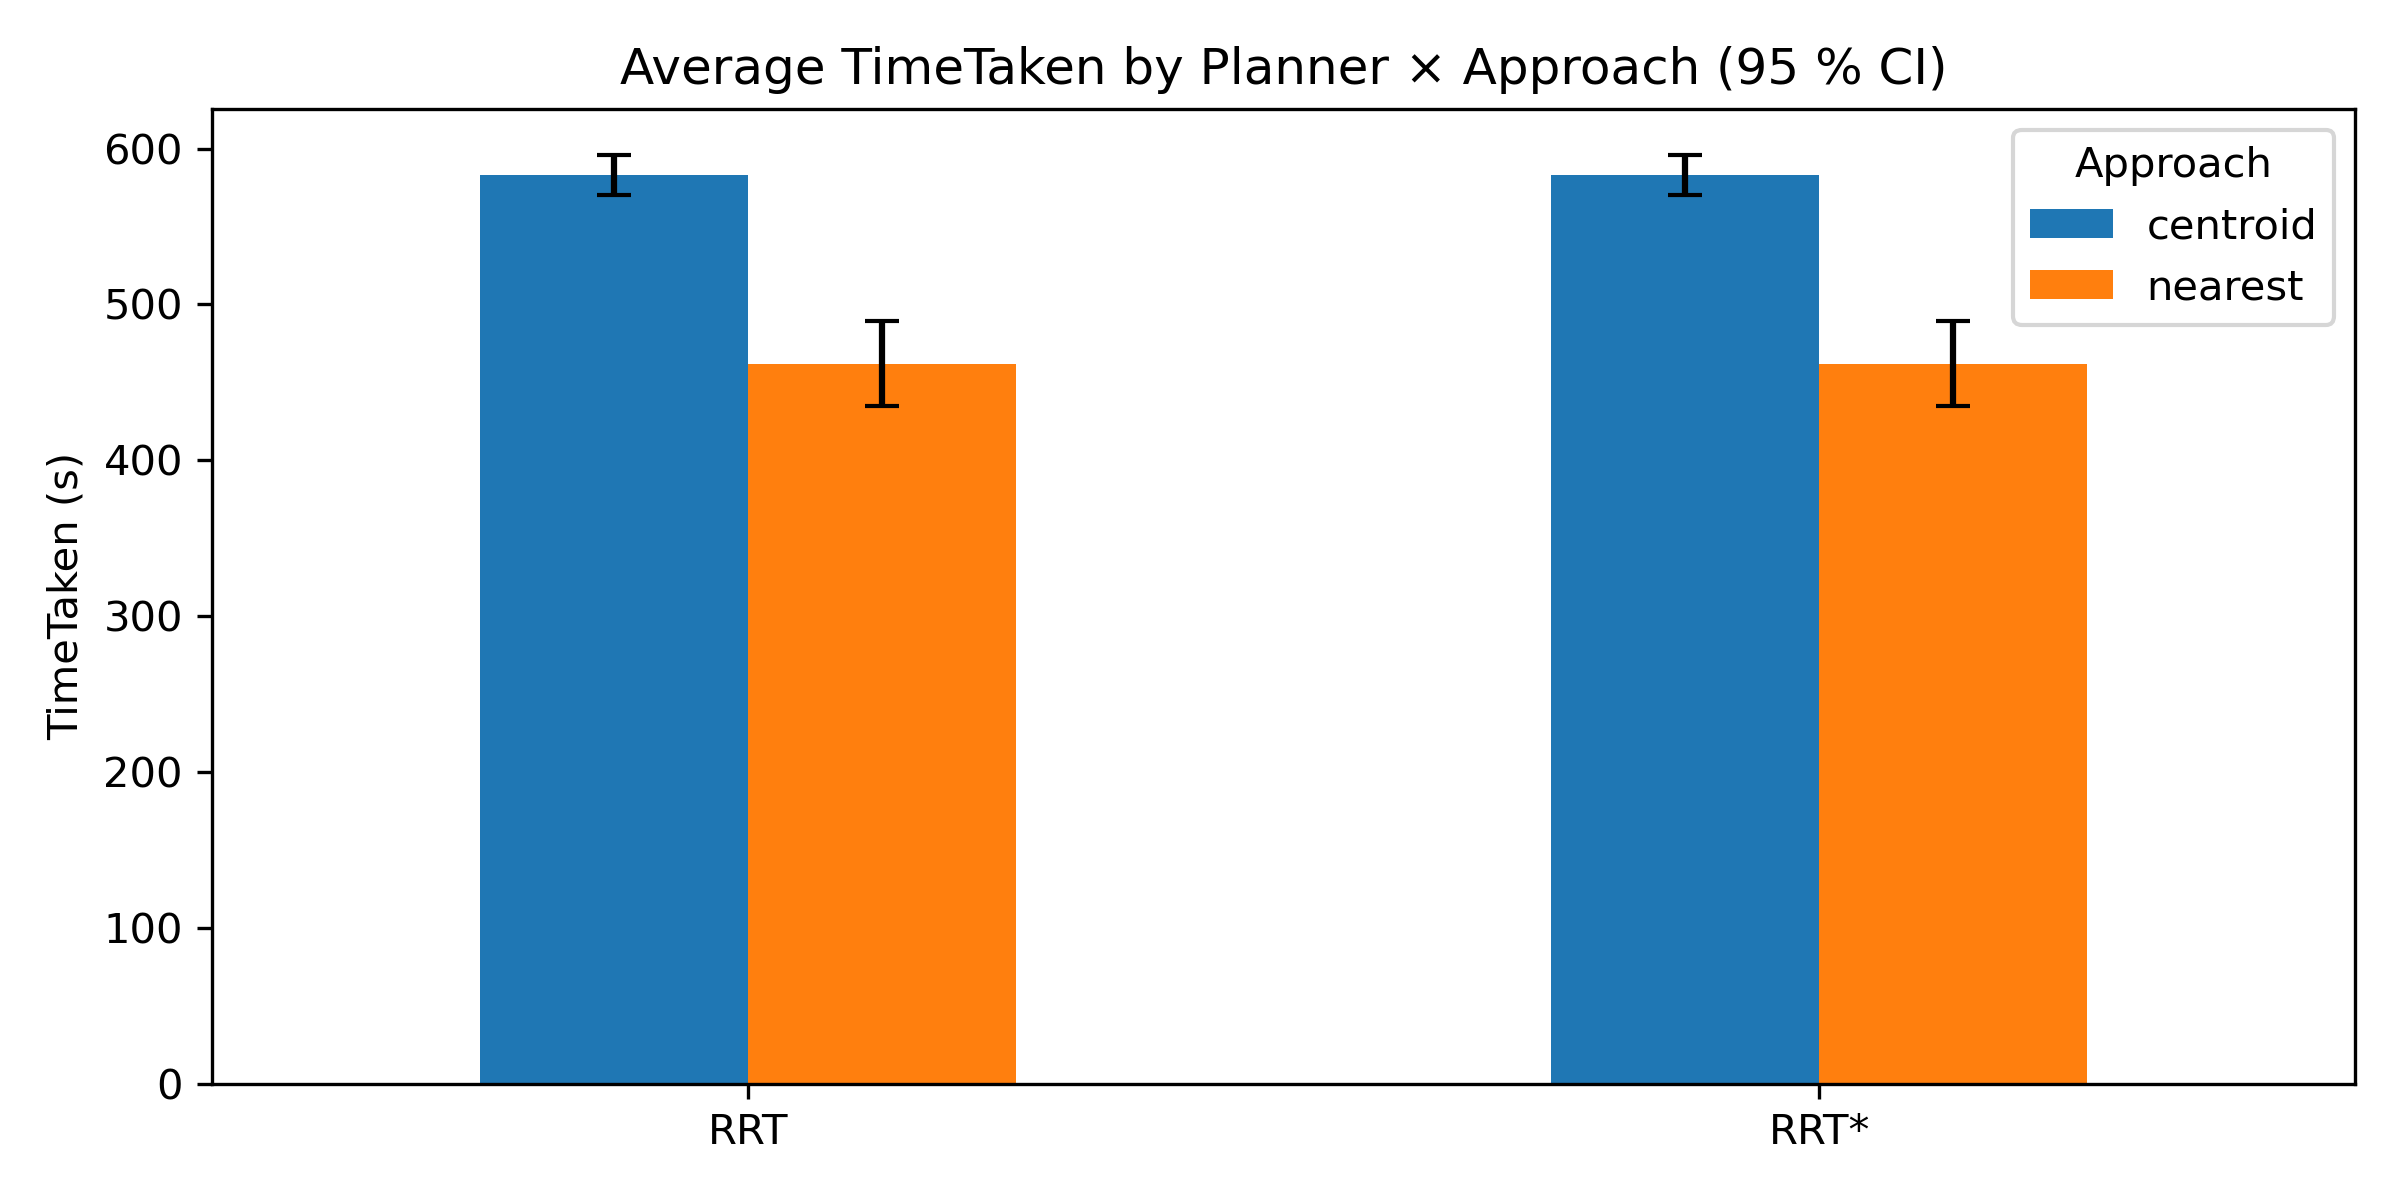
\includegraphics[width=0.75\textwidth]{figures/avg_time_taken.png}
    \caption{Average TimeTaken for each scenario, grouped by planner (RRT vs.\ RRT*) 
             and survivor assignment (nearest vs.\ centroid). The x-axis labels 
             combine map size, building density, and survivor count.}
    \label{fig:avg_time_taken}
\end{figure}

\noindent
In \figurename~\ref{fig:avg_time_taken}, each bar corresponds to the mean rescue time
across three random seeds for a specific combination of:
\emph{(MapWidth, Buildings, Survivors) $\times$ \{RRT or RRT*\} $\times$ \{nearest or centroid\}}.
Notable observations include:
\begin{itemize}
    \item \textbf{Large maps (500$\times$500)} combined with \textbf{dense buildings (60)}
          often lead to longer times or timeouts, particularly under \emph{centroid}.
    \item \textbf{RRT vs.\ RRT*} does not drastically change final times in most scenarios,
          suggesting that standard RRT finds a feasible path quickly, while RRT* 
          may not have enough rewiring time or the environment is not complex enough 
          to leverage RRT*'s optimality advantage.
\end{itemize}

\subsection{Fraction of Survivors Rescued}
\begin{figure}[H]
    \centering
    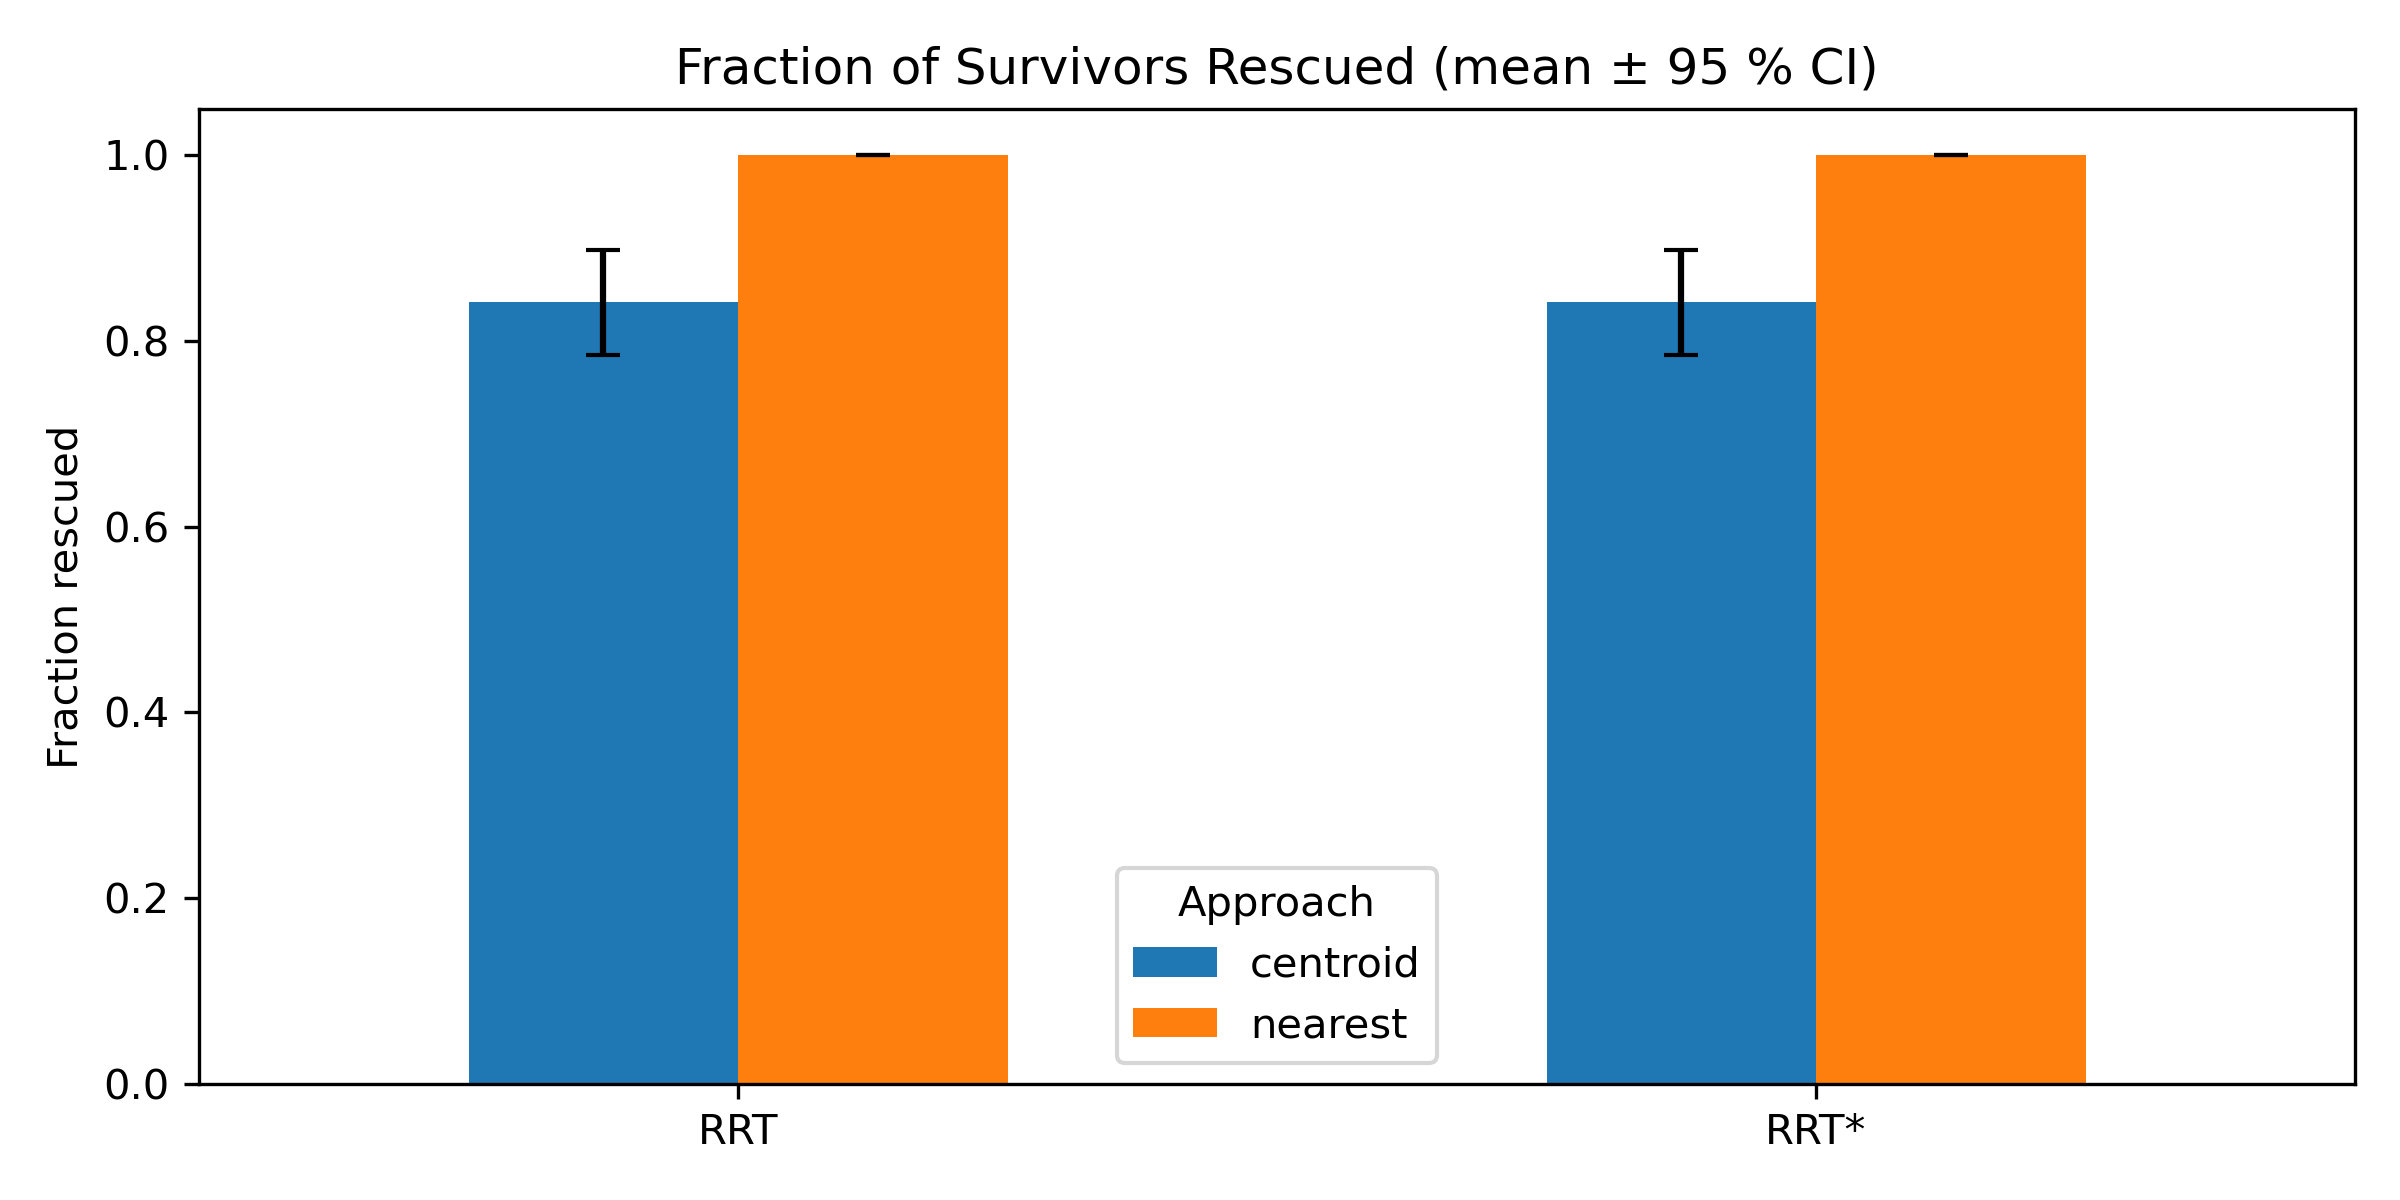
\includegraphics[width=0.75\textwidth]{figures/fraction_rescued.png}
    \caption{Mean fraction of survivors rescued by each scenario. Values below 1.0 
             indicate incomplete rescues within 600\,s (partial success).}
    \label{fig:fraction_rescued}
\end{figure}

\noindent
\figurename~\ref{fig:fraction_rescued} shows the \emph{average fraction of survivors}
rescued across seeds in each scenario. We see:
\begin{itemize}
    \item \textbf{Smaller building counts (30)} often yield fraction~=~1.0,
          i.e.\ all survivors are rescued before time runs out.
    \item With \textbf{25 survivors} and \textbf{60 buildings}, centroid-based approaches 
          occasionally result in partial rescues (fraction < 1.0) in large maps, 
          indicating that 600\,s was insufficient to reach all survivors under 
          less localized assignment logic.
    \item RRT vs.\ RRT* rarely shifts the fraction rescued drastically, 
          aligning with the time data in \figurename~\ref{fig:avg_time_taken}.
\end{itemize}

\subsection{Aerial Drone Distances}
\begin{figure}[H]
    \centering
    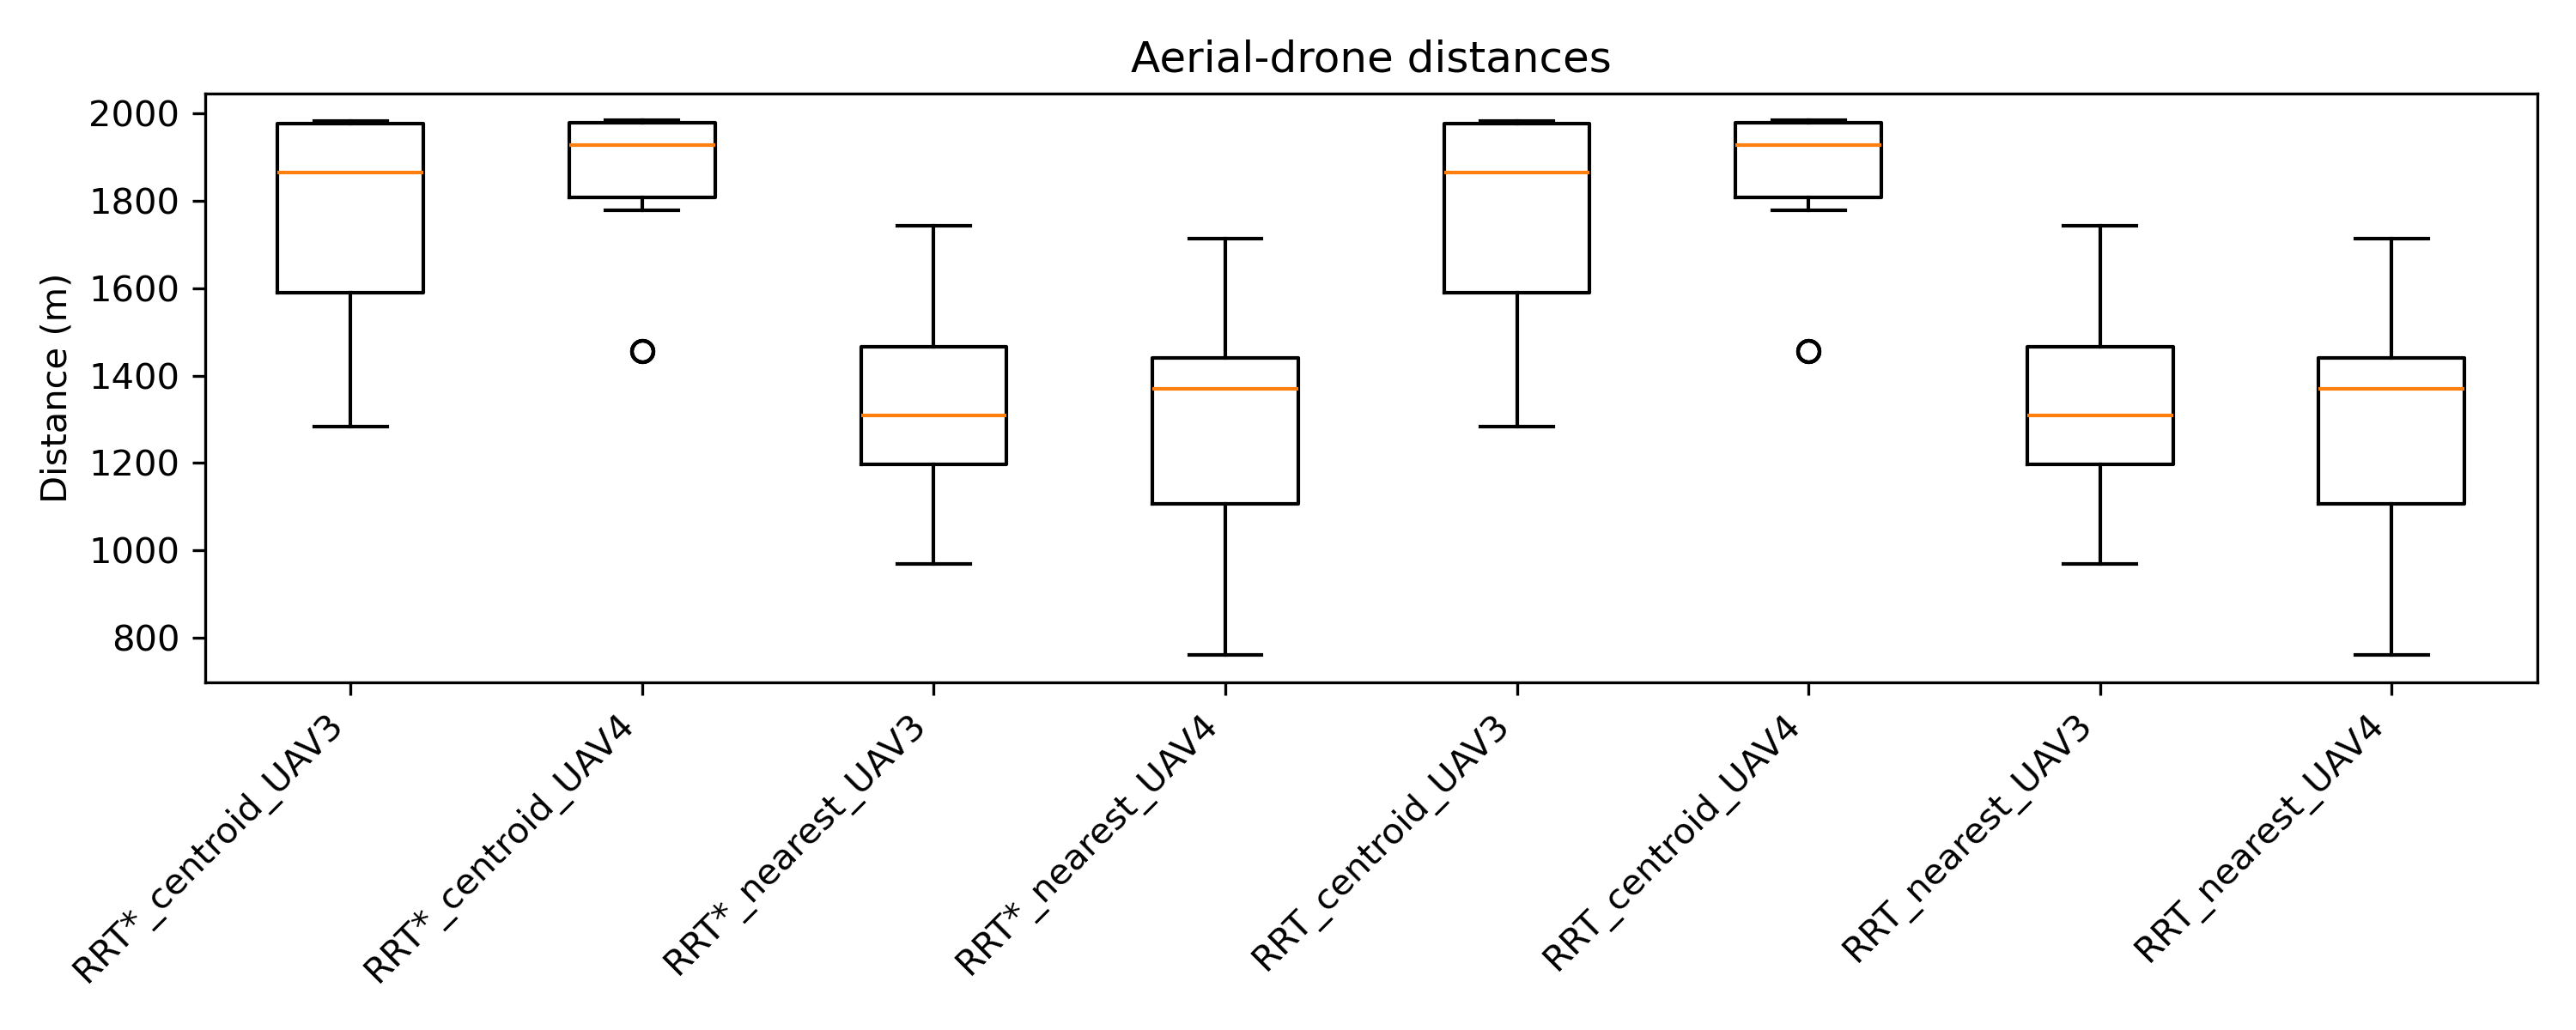
\includegraphics[width=0.75\textwidth]{figures/aerial_distance_box.png}
    \caption{Box plot of distance traveled by the aerial drones (UAV3 and UAV4), 
             grouped by RRT vs.\ RRT* and approach. Each box spans the quartiles 
             over seeds and all scenario variations (map size, building count, survivors).}
    \label{fig:aerial_distance_box}
\end{figure}

\noindent
\figurename~\ref{fig:aerial_distance_box} shows how UAV3 and UAV4 (both aerial) 
tend to travel further than ground vehicles. Key insights:
\begin{itemize}
    \item \textbf{Centroid approaches} often produce higher outliers, as a drone 
          repeatedly relocates to new centroid positions, especially in larger or denser maps.
    \item Some runs with \textbf{RRT*} have a slightly narrower distribution, 
          suggesting the aerial path might be fractionally more optimal.
    \item UAV3 consistently travels more than UAV4 in some seeds, implying it 
          often picks up leftover or scattered survivors.
\end{itemize}

\subsection{Ground Vehicle Distances}
\begin{figure}[H]
    \centering
    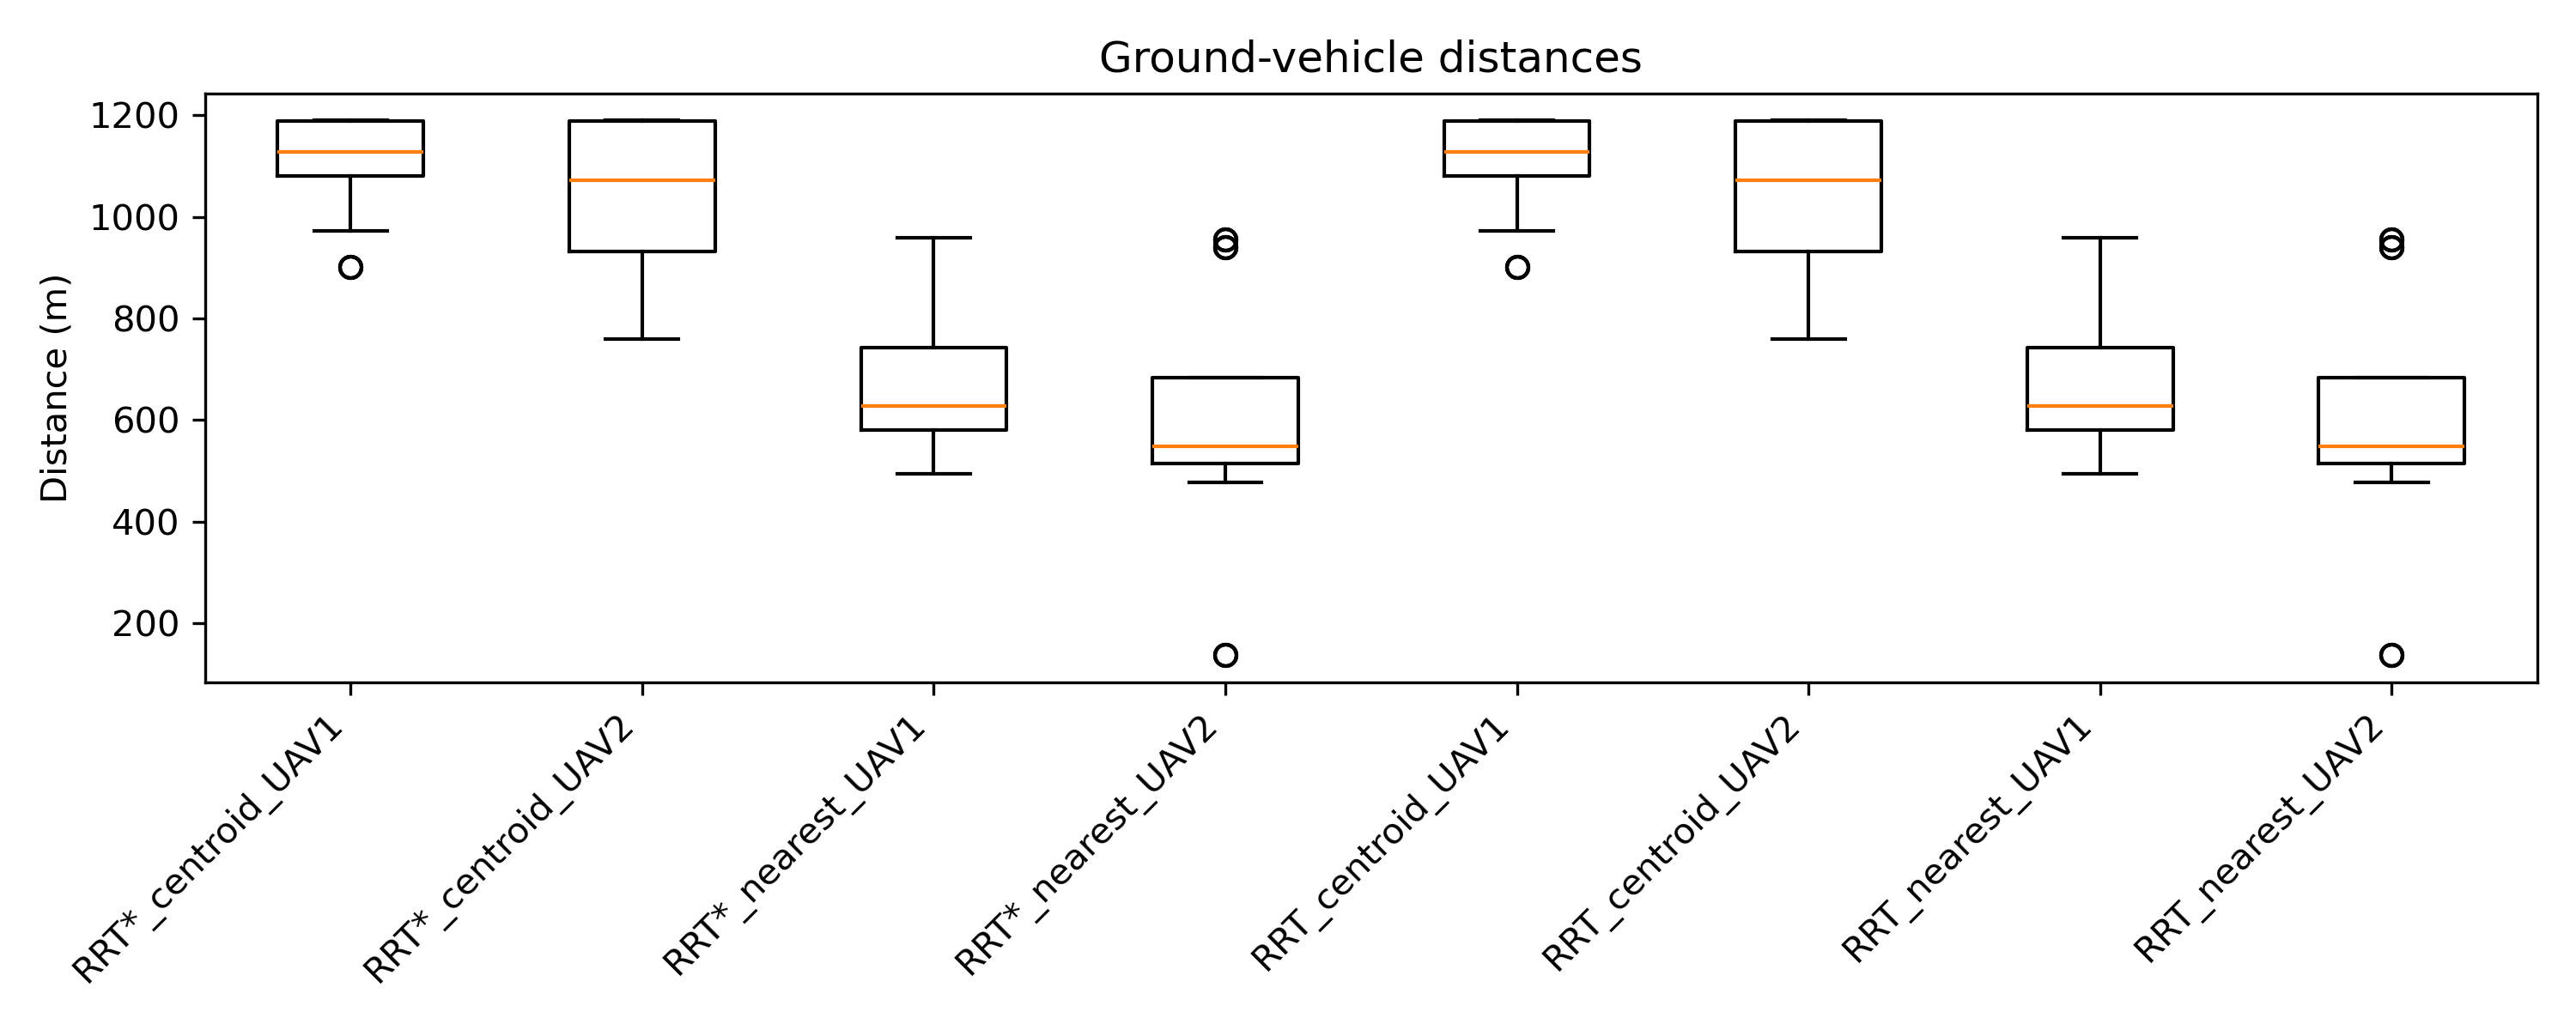
\includegraphics[width=0.75\textwidth]{figures/ground_distance_box.png}
    \caption{Box plot of distance traveled by ground vehicles (UAV1 and UAV2), 
             grouped by RRT vs.\ RRT* and approach.}
    \label{fig:ground_distance_box}
\end{figure}

\noindent
\figurename~\ref{fig:ground_distance_box} highlights that UAV1 and UAV2 generally 
cover fewer kilometers than aerial drones, since they remain in 2D and typically 
handle survivors local to them. In scenarios with \textbf{low building counts}, 
ground vehicles might collectively rescue a fair fraction without needing aerial help. 
Conversely, dense building layouts can hamper ground movement, increasing path length 
variability or stalling partial rescues.

%------------------------------------------------------
\section{Comparative Analysis}
\label{sec:analysis}

\subsection{Nearest vs.\ Centroid}
Across all tested seeds and environment sizes, \emph{nearest-based} assignment 
often yields shorter average mission times, especially in \textbf{large maps} or 
\textbf{high building densities}. Nearest-based logic ensures a quick local 
pickup of survivors without incurring cross-map travel to chase centroid locations, 
which can be detrimental when obstacles force long detours. 

In simpler, smaller maps with fewer buildings, the \emph{centroid} strategy does not 
significantly lag behind nearest. However, it rarely outperforms nearest in a consistent 
way. Some partial rescues occur with centroid, particularly at 25 survivors and 60 buildings.

\subsection{RRT vs.\ RRT*}
Despite RRT*’s theoretical advantage in refining paths, the difference from standard 
RRT is marginal in most scenarios. This suggests:
\begin{enumerate}
    \item \textbf{Time budget (600\,s)} is too short for RRT* to realize 
          substantial rewiring benefits, or 
    \item The environment is already moderately navigable, so a feasible 
          path is found quickly and refining it offers minimal overall rescue-time gain.
\end{enumerate}
In some rare cases, RRT* shows slightly reduced \emph{aerial drone distance} or fractionally 
shorter times, but these were not statistically significant across seeds.

\subsection{Impact of Map Size and Building Density}
Unsurprisingly, a 500$\times$500 area or 60 buildings consistently inflates mission times, 
leads to incomplete rescues, and drives up UAV distance. High obstacle clutter 
limits ground vehicles, shifting more burden to aerial drones, which then must 
criss-cross large spaces. This effect is amplified under \emph{centroid}, as UAVs 
periodically recalculate centroids and relocate.

\subsection{Summary of Findings}
Overall, the data indicate:
\begin{itemize}
    \item \textbf{Nearest approach} is typically the safest choice for fast completion 
          in more challenging scenarios.
    \item \textbf{RRT vs.\ RRT*} differences are minimal under the tested time and 
          environment scales.
    \item \textbf{Map expansions} and \textbf{dense buildings} degrade performance, 
          sometimes leading to partial rescues.
    \item \textbf{Aerial drones} bear the brunt of extended travel in large or 
          cluttered scenarios, while ground vehicles remain more localized.
\end{itemize}
These patterns form a basis for discussing the limitations, possible enhancements, 
and real-world applicability of the system in the subsequent chapters.
%------------------------------------------------------
%------------------------------------------------------
% CHAPTER 6: DISCUSSION
%------------------------------------------------------
\chapter{Discussion}
\label{ch:discussion}

This chapter reflects on the multi-UAV rescue framework in light of the results presented 
in Chapter~\ref{ch:results}. Section~\ref{sec:strengths_weaknesses} reviews the system's 
major strengths and weaknesses, considering both the code architecture and the 
experimental outcomes. Section~\ref{sec:limitations} elaborates on inherent constraints 
of our simulation approach, while Section~\ref{sec:lessons_learned} summarizes key 
insights gained throughout the project.

\section{Strengths and Weaknesses}
\label{sec:strengths_weaknesses}
A principal strength of our system is its \emph{modular} design, as highlighted in 
Chapters~\ref{cha:system_design} and~\ref{cha:implementation}. The distinction between 
environment generation, UAV classes (\texttt{BaseUAV}, \texttt{AerialDrone}, and 
\texttt{GroundVehicle}), and high-level scripts (\texttt{runRescueMission}, 
\texttt{compareApproaches}, \texttt{runExperiments}) allows for straightforward 
extension or modification of each component. In particular, substituting an alternative 
planner (e.g., D* Lite or PRM) or adding specialized vehicle types does not require 
rewriting large sections of the codebase. This architecture proved beneficial when 
enabling both aerial and ground vehicles to operate in parallel, each referencing the 
same environment representation but validated in 2D vs.\ 3D.

From a performance perspective, the results in Chapter~\ref{ch:results} demonstrate 
that \emph{nearest-based} survivor assignment is often robust and efficient, especially 
under higher building densities or larger maps. By contrast, the \emph{centroid} approach, 
while conceptually promising for balanced coverage, sometimes yielded partial rescues 
when the environment became large or cluttered. Thus, the multi-assignment framework 
exhibited both efficiency and flexibility, but remains sensitive to the chosen heuristic.

In terms of weaknesses, RRT* rarely showed a marked improvement over standard RRT, 
suggesting that within a 600\,s mission time, incremental rewiring did not confer 
significant benefits. The overhead of RRT* planning, especially in a 3D environment 
with many expansions, may impede the mission enough that the overall time advantage 
is lost. A further weakness of the current system is its reliance on a \emph{static} 
environment assumption: buildings do not collapse or move, and survivors remain 
stationary. Though suitable for a proof-of-concept, it limits real-world realism 
(citation needed). Additionally, k-means assignment, while implemented in the code, 
was not fully integrated or utilized in final experiments due to partial reliability 
issues.

\section{Limitations}
\label{sec:limitations}
While the simulation framework achieves a broad set of objectives, several limitations 
should be acknowledged:

\paragraph{Static Obstacles and Survivors.}
No dynamic or moving obstacles are modeled, nor do survivors shift location. In real 
disaster scenarios, rubble can shift, additional hazards can arise, or survivors may 
attempt to relocate (citation needed). Such dynamics would demand real-time replanning.

\paragraph{Perfect Communication.}
All UAVs are assumed to share information instantaneously, ignoring factors like 
network latency, bandwidth constraints, or communication failures. Real-world 
decentralized or partially connected networks would create new complexities (citation needed).

\paragraph{Limited UAV Fleet and Speeds.}
We employ exactly two ground vehicles and two aerial drones, each with fixed speeds. 
Though sufficient to demonstrate multi-agent task allocation, larger or more diverse 
fleets might unveil further coordination challenges, such as interference or 
load-balancing difficulties.

\paragraph{Finite Time Budget.}
Experiments used a 600\,s limit, beyond which runs were considered incomplete. Certain 
scenarios (large map, 60 buildings, 25 survivors) frequently timed out, indicating 
that mission success strongly depends on how quickly feasible paths can be found and 
survivors assigned. Longer time budgets might reveal whether RRT* eventually outperforms RRT.

\paragraph{Simplified Planner Comparison.}
Our code primarily compares standard RRT and RRT*. While these capture significant 
differences in sampling-based methods, other algorithms (PRM, A*, D*) may react 
differently to dense or high-dimensional spaces. Extending the code to additional 
planners would further enrich the comparative insights.

\section{Lessons Learned}
\label{sec:lessons_learned}
Across the implementation and experimental phases, several valuable lessons emerged:

\paragraph{Feasible Paths Often Trump Optimality.}
One clear takeaway is that in a time-critical rescue context, a quickly discovered 
feasible path frequently outperforms a slower search for an optimal one, especially 
when facing partial or uncertain environment information (citation needed). Our 
results confirm that under realistic time budgets, RRT's speed often suffices.

\paragraph{Multi-Agent Tasking is Key.}
While single UAV strategies can be effective for small areas or low building densities, 
the partial rescues encountered in large or cluttered scenarios highlight the need 
for robust, perhaps dynamic, multi-agent allocation. Our nearest-based approach 
demonstrated strong performance, but more advanced strategies—like auction-based 
methods—may be necessary for truly large fleets or dynamic obstacles.

\paragraph{Environment Generation for Testing.}
The \emph{procedural} environment model allowed quick iteration across seeds and 
densities, revealing which parameter combinations cause timeouts. Future expansions 
could incorporate real-world topologies (e.g., satellite data), bridging the gap 
between simulation and field testing.

\paragraph{Modular Design Eases Comparisons.}
Finally, the modular code structure simplified the integration of different path 
planners and assignment strategies, a principle that future rescue simulators 
could adopt. Clear separation of environment, UAV classes, and mission script 
logic not only facilitates experimentation but also clarifies how each subsystem 
interacts and impacts final outcomes.

Overall, these lessons underscore that real-time multi-UAV rescue scenarios demand 
both rapid feasibility (RRT) and efficient assignment heuristics (nearest or otherwise) 
that match the environment's size, clutter level, and available time.
%------------------------------------------------------
% CHAPTER 7: CONCLUSION AND FUTURE WORK
%------------------------------------------------------
\chapter{Conclusion \& Future Work}
\label{ch:conclusion}

\section{Summary of Achievements}
Over the course of this project, we developed a comprehensive multi-UAV rescue simulation
that integrates both ground vehicles (operating in 2D) and aerial drones (operating in 3D).
A key accomplishment is the \emph{modular} software design that cleanly separates
environment generation, UAV classes, path planning, and top-level mission scripts.
This architecture enabled us to seamlessly compare and switch between RRT vs.\ RRT*,
as well as evaluate different survivor assignment heuristics (nearest vs.\ centroid).

Through extensive experimentation (96 runs) spanning various map sizes, building densities,
and survivor counts, we gathered performance metrics such as rescue time, fraction of
survivors rescued, and UAV travel distance. Our results showed that:
\begin{itemize}
    \item \textbf{Nearest-based} assignments typically lead to faster completion than
          centroid in larger or cluttered environments.
    \item \textbf{RRT*} rarely offers a substantial advantage over standard RRT within
          our 600\,s limit, implying that a quick, feasible path is generally more
          beneficial than an incrementally refined one for time-critical rescues.
    \item \textbf{Aerial drones} shoulder the heaviest travel load in complex scenarios,
          while ground vehicles effectively handle local survivors if obstacles are not
          too dense.
\end{itemize}
Overall, we have demonstrated that even relatively simple sampling-based planners and
heuristic assignment methods can effectively coordinate multi-vehicle rescues in
procedurally generated static environments.

\section{Future Extensions}
Although the current system serves as a valuable testbed, several avenues exist to
broaden its realism and applicability:
\begin{itemize}
    \item \textbf{Dynamic and Real-Time Updates}: Incorporating moving survivors or
          shifting rubble piles would require on-the-fly replanning and sensor-based
          occupancy map updates, mirroring real-world disaster volatility.
    \item \textbf{Advanced Task Allocation}: While nearest-based and centroid heuristics
          suffice for moderate scenarios, large-scale rescues could benefit from auction-based
          or market-based assignments that handle greater team sizes and dynamic constraints.
    \item \textbf{Additional Planners \& Approaches}: Extending beyond RRT or RRT*
          to algorithms like PRM, D*, or machine-learning-driven planners could
          uncover more optimal or robust solutions, particularly for high-density
          or partially unknown environments.
    \item \textbf{Communication Constraints}: The assumption of perfect, instant
          communication simplifies coordination but diverges from real-world
          network limitations. Implementing bandwidth, range, and latency constraints
          would provide a more realistic challenge for multi-UAV rescue operations.
    \item \textbf{Hardware-in-the-Loop Testing}: Finally, connecting this simulator
          to actual drone or ground-robot hardware would verify whether the software
          performance translates reliably into the physical domain, paving the way
          for partial or fully realistic field tests.
\end{itemize}

\section{Final Remarks}
In conclusion, this project underscores the promise and complexity of multi-UAV rescue
systems. By uniting aerial and ground vehicles under a common simulation framework,
employing sampling-based planners, and trialing multiple survivor assignment strategies,
we have established a baseline for both feasibility and performance in static, cluttered
settings. Moreover, our findings highlight that even straightforward approaches can
produce successful outcomes in a time-sensitive rescue scenario, provided a feasible
path is discovered quickly and survivors are assigned prudently. We hope this work
serves as a foundation for ongoing innovation in robotic disaster response, culminating
in faster, safer, and more efficient rescue operations worldwide.
%------------------------------------------------------
% REFERENCES
%------------------------------------------------------


%------------------------------------------------------
% APPENDICES (OPTIONAL)
%------------------------------------------------------
%\appendix
%\chapter{Extra Figures or Code}
% If you want to include large code listings or additional figures,
% you can place them here so they don't clutter the main text.

\bibliographystyle{plain}   % or IEEEtran etc.
\bibliography{references}   % ← matches references.bib


\end{document}